\documentclass[../../course]{subfiles}

\renewcommand\thesection{\arabic{section}}


\begin{document}

\def\freqXOne{28}
\def\freqXTwo{56}
\def\freqXThree{56.1}

\section{Taking DTFT of the Complex Sequences} \label{sec:wrkTakingDTFTCplxSeqs}

In the previous section, we generated a bunch of \emph{Complex Sequences}. And
picked $4$ sequences for further analysis. In this section we will be taking
\textsc{DTFT} of those sequences. But before that, we need to take a look at what
a \textsc{DTFT} is and how to elagently compute it using python.

\subsection{Discrete Time Fourier Transform}

Discrete Time Fourier Transform, aka, \textsc{DTFT} transforms \emph{discrete time}
samples into a \emph{continous} signal in the \emph{frequency} domain. \textsc{DTFT}
is basically a special case of another transform known as $\mathcal{Z}$\textsc{-transform}.
$\mathcal{Z}$\textsc{-transform} can be mathematically described as,

\begin{align}
    X(z) = {\mathcal{Z}}\{x[n]\} = \sum_{n = - \infty}^{\infty} x[n] z^{-n}
\end{align}

where,

\begin{itemize} [label=]

    \item ${\mathcal{Z}}\{x[n]\}$: is the $\mathcal{Z}$\textsc{-transform}.
    \item $x[n]$: is the input sequence, which was sampled with a
        particular \emph{sampling frequency}, $f_{s}$.
    \item $z$: is a \emph{complex number}, in the form $A e^{-j \omega}$.

        where,

        \begin{itemize} [label=]
            \item $A$: is the \emph{real part} or the \emph{amplitude}.
            \item $\omega$: is the \emph{complex argument} in radians.
        \end{itemize}

\end{itemize}

\textsc{DTFT} is a special case of $\mathcal{Z}$\textsc{-transform}, where we take $A$
as $1$. Mathematically, we can describe \textsc{DTFT} as,

\begin{align}
    X(e^{j \omega}) &= X(z) |_{z = e^{j \omega}} \\
    &= \sum_{n = - \infty}^{\infty} x[n] z^{-n} \Big|_{z = e^{jw}} \\
    &= \sum_{n = - \infty}^{\infty} x[n] e^{-j w n} \label{eqn:dtftOmega}
\end{align}

Where $\omega$ can be substituted with $2 \pi f$, then the \textsc{DTFT} becomes,

\begin{align}
    X(e^{j 2 \pi f}) &= \sum_{n = - \infty}^{\infty} x[n] e^{-j 2 \pi f n}
    \label{eqn:dtftFreq}
\end{align}

Now eq. (\ref{eqn:dtftOmega}) becomes a function of \emph{frequency} $f$
instead of \emph{angular frequency} $\omega$. One thing to \textsc{note} is that,
\emph{sweeping} $f$ in eq. (\ref{eqn:dtftFreq}) from $0$ to $1$ will result in same
output as \emph{sweeping} $\omega$ in eq. (\ref{eqn:dtftOmega}) from $0$ to $2 \pi$.
Another interesting thing about this \emph{transform} is that the $e^{-1j \pi f n}$ will
\emph{scales} and \emph{wraps} the \emph{frequencies} from $0$ to $\infty$ around
the \textsc{Unit Circle} in the $\mathcal{Z} \textsc{-plane}$. This will become
important as we compute the \textsc{DTFT}s. The Figure \ref{fig:wrapFreqUnitCircle}
attempts to visualizes this interesting concept.

\begin{figure}
    \centering
    \adjustbox{max width = 1\textwidth} {
        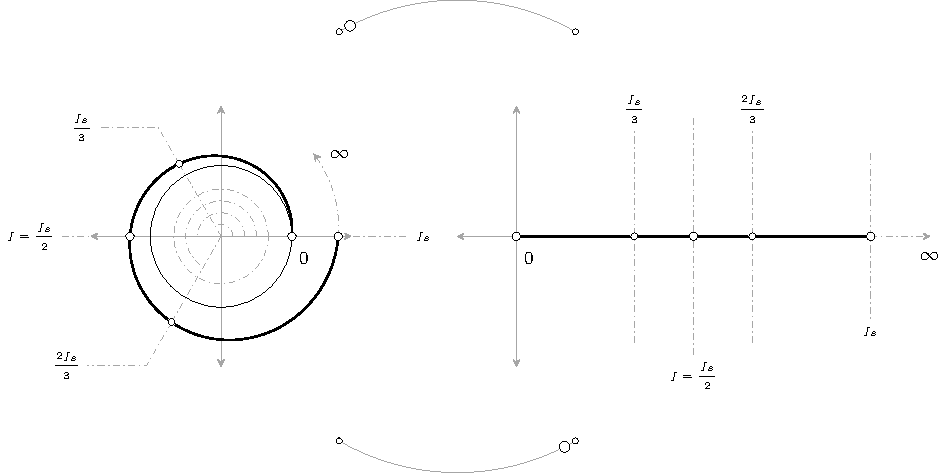
\includegraphics[height = 1\textheight] {tikzpics/epicWrapFreqUnitCircle.pdf}
    }
    \captionof{figure} {
        Wrapping frequencies around the \textsc{Unit Circle} in $\mathcal{Z}\textsc{-plane}$
    }
    \label{fig:wrapFreqUnitCircle}
\end{figure}

\subsection{Implementing DTFT using Python}

We essentially need to take \textsc{DTFT} of several\footnote{actually $4$, still
more than $1$} sequences. So it will be handy to implement a \emph{factory}, that
will take a \emph{sequence} and returns a \emph{dtft function} that can be called
with different \emph{frequencies} and returns it's corresponding value. Let us call
this \emph{function} the \mintinline{python}{dtft_factory}.

%python/dtft_factory.py%
\begin{minted}[breaklines, autogobble, mathescape] {python}
    import numpy as np

    def dtft_factory(cplx_seq):

        def dtft(freq):
            sum = 0
            # see eq. ($\ref{eqn:dtftFreq}$)
            for n, cplx in enumerate(cplx_seq):
                sum = sum + cplx * np.exp(-1j * 2 * np.pi * freq * n)
            return sum

        return dtft
\end{minted}

Now, let's implement another \emph{function} that will returns another
\emph{function}\footnote{yes, ofcourse.} that can be called with $n = 0, 1, 2, ...$
to generate the \emph{sequence} with specified \emph{sampling frequency}, \emph{real}
and \emph{imaginary} parts. Let's call this \emph{function} \mintinline{python}{cplx_factory}

%python/cplx_factory.py%
\begin{minted}[breaklines, autogobble, mathescape] {python}
    import numpy as np

    def cplx_factory(samp_freq, real_freq, imag_freq):
        samp_period = 1 / samp_freq
        return lambda n: np.sin(
            2 * np.pi * real_freq * (n * samp_period)
        ) + 1j * np.sin(
            2 * np.pi * imag_freq * (n * samp_period)
        )
\end{minted}

Let's implement yet another \emph{function} that will make our life easier by
\emph{mixing} and \emph{generating} the \textsc{DTFT} for two given \emph{frequencies}\footnote{one
as \emph{real} and one as \emph{complex}}. As depicted in Figure \ref{fig:wrapFreqUnitCircle}
we only need to evaluate the dtft from $0$ to $1$ range\footnote{in the case
of eq. (\ref{eqn:dtftFreq}).} and need to \emph{rescale} it back.

%python/gen_dtft_seq.py%
\begin{minted}[breaklines, autogobble, mathescape] {python}
    def gen_dtft_seq(
        samp_count, samp_freq, real_freq, imag_freq, dtft_samp_count
        ):

        cplx_fn = cplx_factory(
            samp_freq = samp_freq,
            real_freq = real_freq,
            imag_freq = imag_freq
        )

        cplx_seq = np.ndarray(samp_count, dtype = np.cdouble)

        for i in range(samp_count):
            cplx_seq[i] = cplx_fn(i)

        freq = np.linspace(0, 1, dtft_samp_count)

        dtft_fn = dtft_factory(cplx_seq = cplx_seq)
        dtft_seq = dtft_fn(freq)

        # scaling back the freq from ($0$ - $1$) to ($0$ - $f_{s}$)
        return freq * samp_freq, dtft_seq, cplx_seq
\end{minted}

Now we could just call \mintinline{python}{gen_dtft_seq} with appropriate \emph{arguments}
and it will return the \mintinline{python}{dtft_seq} and its corresponding \emph{frequencies}.
Let's take a bunch of \textsc{DTFT}s with different \emph{sampling frequencies}.

%python/taking_dtft.py%
\begin{minted}[breaklines, autogobble, mathescape] {python}
    import pandas as pd

    X = 28

    cplx_seqs = [
        {
            "name": "complex_a",
            "real_freq": X,
            "imag_freq": X,
            # we will fill this later, for taking 64 point DTFT
            "sequences": {},
        },
        {
            "name": "complex_b",
            "real_freq": X,
            "imag_freq": 2 * X,
            "sequences": {},
        },
        {
            "name": "complex_c",
            "real_freq": X,
            "imag_freq": (2 * X) + 0.1,
            "sequences": {},
        },
        {
            "name": "complex_f",
            "real_freq": 2 + X,
            "imag_freq": (2 * X) + 0.1,
            "sequences": {},
        },
    ]

    samp_freqs = {
        "normal":           int(4 * X),
        "slightly_greater": int(4 * X + 6),
        "much_greater":     int(4 * X * 2),
        "much_lesser":      int(4 * X / 2),
    }

    samp_count = 32

    dtft_samp_count = 2000

    for cplx in cplx_seqs:

        for samp_freq in samp_freqs:

            freq, dtft_seq, cplx_seq = gen_dtft_seq(
                samp_count = samp_count,
                samp_freq = samp_freqs[samp_freq],
                real_freq = cplx["real_freq"],
                imag_freq = cplx["imag_freq"],
                dtft_samp_count = dtft_samp_count
            )

            # keeping generated sequences for taking 64 point DTFT
            cplx["sequences"][samp_freq] = cplx_seq

            data = pd.DataFrame(
                data = {
                    "real": dtft_seq.real,
                    "imag": dtft_seq.imag,
                },
                index = freq
            )

            data.to_csv(
                "../data/dtft_" + cplx["name"] + "_" + samp_freq + ".csv",
                sep = " ", index_label = "freq"
            )
\end{minted}

We have generated \textsc{DTFT}s for our \emph{sequences} with
different \emph{sampling frequencies}, and \mintinline{python} {cplx_seqs}
dictionary has all those generated \emph{input sequences}. Now we need
to pad them with $32$ zeros and find the \textsc{DTFT}s of those sequences.
Let's quickly implement another \emph{function} for that. Let it be
\mintinline{python}{gen_dtft_seq_64}.

%python/gen_dtft_seq_64.py%
\begin{minted}[breaklines, autogobble, mathescape] {python}
    def gen_dtft_seq_64(
        cplx_seq, samp_freq, dtft_samp_count
        ):

        cplx_seq = np.concatenate(
            [cplx_seq, np.zeros(32, dtype = np.cdouble)]
        )

        freq = np.linspace(0, 1, dtft_samp_count)

        dtft_fn = dtft_factory(cplx_seq = cplx_seq)
        dtft_seq = dtft_fn(freq)

        # scaling back the freq from ($0$ - $1$) to ($0$ - $f_{s}$)
        return freq * samp_freq, dtft_seq, cplx_seq
\end{minted}

Now let's take the \textsc{DTFT}s of those sequences using this
\mintinline{python}{gen_dtft_seq_64}.

%python/taking_dtft_64.py%
\begin{minted}[breaklines, autogobble, mathescape] {python}
    dtft_samp_count = 2000

    for cplx in cplx_seqs:
        for seq_name in cplx["sequences"]:
            freq, dtft_seq, _ = gen_dtft_seq_64(
                cplx_seq = cplx["sequences"][seq_name],
                samp_freq = samp_freqs[seq_name],
                dtft_samp_count = dtft_samp_count
            )

            data = pd.DataFrame(
                data = {
                    "real": dtft_seq.real,
                    "imag": dtft_seq.imag,
                },
                index = freq
            )

            data.to_csv(
                "../data/dtft_" + cplx["name"] + "_" + seq_name + "_64.csv",
                sep = " ", index_label = "freq"
            )
\end{minted}

\subsection{DTFT of Complex A} \label{ssec:dtftCplxA}

\begin{figure}
    \centering
    \adjustbox{max width = 1\textwidth} {
        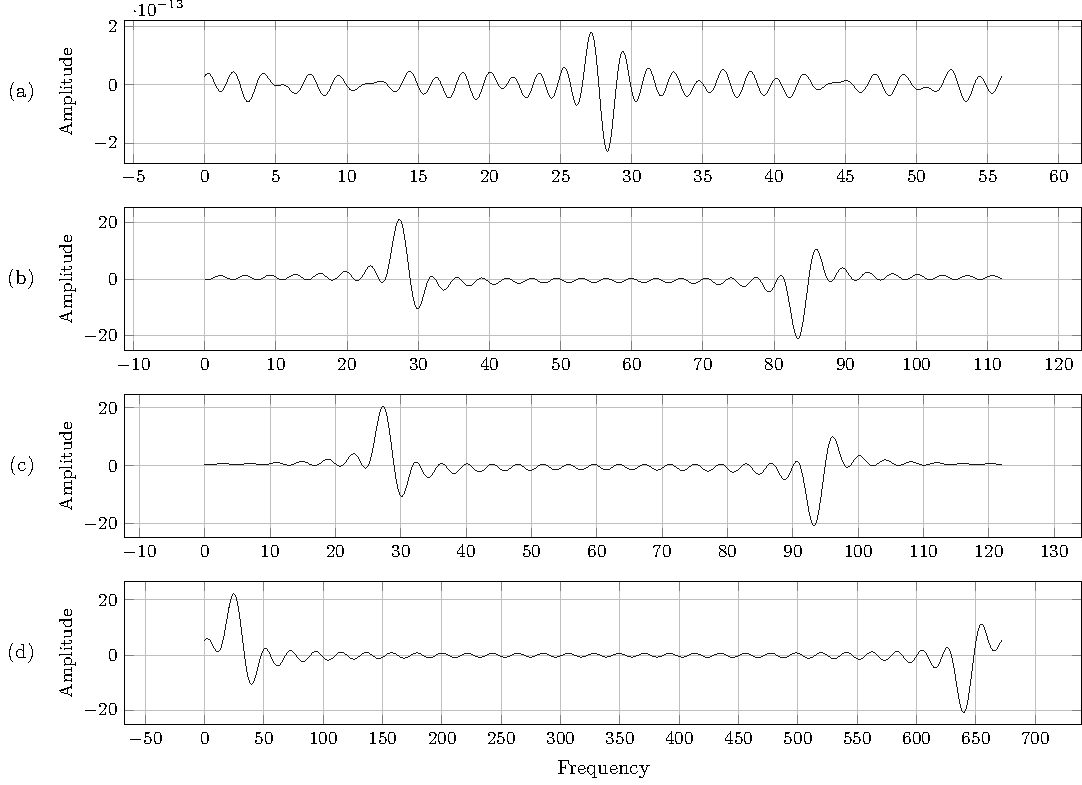
\includegraphics[height = 0.8\textheight] {tikzpics/plotDtftComplexA.pdf}
    }
    \captionof{figure} {Plot of \textsc{DTFT} of \textsc{Complex A}}
    \label{plt:dtftComplexA}
\end{figure}



%% In Sections \ref{sec:wrkGenSeqs} and \ref{sec:wrkGenCompSeqs}, we did

%%% A
%%% $x_{1} + j x_{1}$
%
%\textbf{Sequence:} $\sin(2 \pi \freqXOne t) + j \sin(2 \pi \freqXOne t)$
%
%%% B
%%% $x_{1} + j x_{2}$
%
%\textbf{Sequence:} $\sin(2 \pi \freqXOne t) + j \sin(2 \pi \freqXTwo t)$
%
%%% C
%%% $x_{1} + j x_{3}$
%
%\textbf{Sequence:} $\sin(2 \pi \freqXOne t) + j \sin(2 \pi \freqXThree t)$
%
%%% F
%%% $x_{2} + j x_{3}$
%\textbf{Sequence:} $\sin(2 \pi \freqXTwo t) + j \sin(2 \pi \freqXThree t)$
%
%%%  a, b, c, f


\end{document}
